% Final report. Build: .venv/bin/python scripts/final_report.py && cd report/final && tectonic final_report.tex
% All numbers in generated tables and \Macros come from scripts/final_report.py (full-run artifacts).
\documentclass[conference]{IEEEtran}
\usepackage[utf8]{inputenc}
\usepackage[T1]{fontenc}
\usepackage{graphicx,booktabs,amsmath,amssymb,xcolor,tikz,hyperref,cite,array}
\usetikzlibrary{arrows.meta,positioning}
\hypersetup{colorlinks=true,linkcolor=blue!50!black,citecolor=blue!50!black,urlcolor=blue!50!black}
\graphicspath{{figures/}}
\newcommand{\BaseAcc}{43.2}
\newcommand{\BaseNum}{40.2}
\newcommand{\ScAcc}{53.2}
\newcommand{\ScN}{20}
\newcommand{\PotAcc}{48.2}
\newcommand{\PotNum}{50.4}
\newcommand{\CsAcc}{51.2}
\newcommand{\CcAcc}{51.3}
\newcommand{\VerAcc}{63.2}
\newcommand{\FullAcc}{65.3}
\newcommand{\FullNum}{69.0}
\newcommand{\FullLo}{57.4}
\newcommand{\FullHi}{73.7}
\newcommand{\FullDelta}{+22.1}
\newcommand{\FullTok}{54.1k}
\newcommand{\FullVsSc}{+12.1}
\newcommand{\FullVsScLo}{+4.2}
\newcommand{\FullVsScHi}{+20.5}
\newcommand{\FullVsScP}{0.001}
\newcommand{\FullOnly}{35}
\newcommand{\ScOnly}{12}
\newcommand{\ScMax}{54.7}
\newcommand{\CotTrunc}{40}
\newcommand{\PotTrunc}{37}
\newcommand{\ReproAcc}{13.8}
\newcommand{\ReproStd}{1.9}
\newcommand{\ConTrain}{43.9}
\newcommand{\ConTest}{42.6}
\newcommand{\ConDelta}{-1.3}
\newcommand{\VerN}{10{,}160}
\newcommand{\VerDevAuc}{0.915}
\newcommand{\VerTestAuc}{0.836}
\newcommand{\XgbTestAuc}{0.882}
\newcommand{\SelMaj}{65.8}
\newcommand{\SelPrim}{65.3}
\newcommand{\SelXgb}{67.9}
\newcommand{\SelOracle}{85.3}
\newcommand{\SelRandom}{52.8}
\newcommand{\Ece}{0.063}
\newcommand{\RagMean}{50.9}
\newcommand{\KbEntries}{454}
\newcommand{\RagN}{30}
\newcommand{\RagWithPot}{30.0}
\newcommand{\RagWithRag}{37.9}
\newcommand{\RagWoPot}{51.6}
\newcommand{\RagWoRag}{53.4}
\newcommand{\FixSame}{14.3}
\newcommand{\FixCross}{18.6}
\newcommand{\FixFull}{19.2}
\newcommand{\PotCodeRan}{26}
\newcommand{\PotFallback}{36}
\newcommand{\TotalHours}{54}


\begin{document}
\title{Improving Scientific Reasoning in Vision-Language Models with Code Sandboxes, Agentic
Correction, Learned Verification and Retrieval on mmJEE-Eval}
\author{\IEEEauthorblockN{Arpit Kumar (12340350) \quad Saurav Gupta (12341940)}
\IEEEauthorblockA{Machine Learning course project, IIT Bhilai}}
\maketitle

\begin{abstract}
mmJEE-Eval shows that open vision-language models (VLMs) solve few JEE-Advanced problems and,
when asked to fix their own errors, succeed only 1.1--5.2\% of the time. We wrap a \emph{frozen}
4-bit VLM (Qwen3-VL-8B) in a training-free, inference-time framework with four modules: (A) a
code sandbox for program-of-thought computation, (B) a Critic/Corrector loop that locates the
first wrong step and re-derives from it, (C) a learned solution verifier, the only trained
component, and (D) retrieval of verified worked solutions as exemplars. On the 190-question 2025
held-out set (English and Hindi), Pass@1 rises from \BaseAcc\% for chain-of-thought to
\FullAcc\% for the full framework (\FullDelta{} points, 95\% CI [\FullLo, \FullHi]). At the same
generated-token budget it beats self-consistency by \FullVsSc{} points (CI [\FullVsScLo,
\FullVsScHi], McNemar $p{=}$\FullVsScP). Our analysis shows where the gain comes from: code
lifts Numerical accuracy, step-localised correction fixes \FixCross\% of detected errors (vs.\
1.1--5.2\% in the paper), and most of the large jump comes from selecting among a diverse pool of
code-based and corrected candidates. On 2025 the learned verifier selects as well as majority
voting but not better, and retrieval helps only the few questions with a close match. A
contamination check finds no advantage on older exam years.
\end{abstract}

% ----------------------------------------------------------------------------------------------
\section{Introduction}
JEE-Advanced questions combine a diagram, multi-step physical or chemical reasoning and exact
numerical answers. mmJEE-Eval~\cite{mmjee} turns 1{,}460 of them (2019--2025, English and Hindi)
into an image-only benchmark. It reports that open VLMs are weak, e.g.\ 12.4\% Pass@1 for
Qwen2.5-VL-7B on 2025, and that their single-pass self-correction rarely turns a detected error
into a correct answer (1.1--5.2\%). The paper releases an evaluation harness but no method to
close the gap.

Our SOP proposed to attack the two diagnosed weaknesses, numerical computation and turning
detection into a fix, \emph{at inference time}, without fine-tuning the VLM. We make the
following contributions:
\begin{itemize}
\item A complete, tested framework around a frozen 4-bit VLM: code sandbox (PoT), Critic/Corrector
loop, learned verifier and retrieval, evaluated additively as in SOP Table~I against
compute-matched self-consistency (SC)~\cite{selfconsistency}.
\item A harness that reuses the paper's scoring byte-for-byte and reproduces its Qwen2.5-VL-7B
number (\ReproAcc\% vs.\ 12.4\%).
\item Results on all 190 test questions: \BaseAcc\%$\to$\FullAcc\% Pass@1, \FullVsSc{} points
over SC at equal compute, with cluster-bootstrap CIs and McNemar tests.
\item An analysis of \emph{where} the gain comes from (code use, correction dynamics, candidate
pool vs.\ selector, retrieval coverage), a contamination check, and an account of the errors we
found and fixed on the way.
\end{itemize}

% ----------------------------------------------------------------------------------------------
\section{Related work}
\textbf{Tool-augmented reasoning.} Program-of-thought~\cite{pot} and PAL~\cite{pal} move
arithmetic out of the language model into an interpreter; we apply this to multimodal problems,
with execution feedback inside the generation.
\textbf{Sampling and voting.} Self-consistency~\cite{selfconsistency} votes over sampled
chains; it is our compute-matched baseline.
\textbf{Self-correction.} Self-Refine~\cite{selfrefine} and CRITIC~\cite{critic} iterate
critique and revision, but intrinsic self-correction often fails without external
signal~\cite{cannotselfcorrect}; we add code execution, step localisation and a cross-model
critic.
\textbf{Verifiers.} Trained outcome and process verifiers~\cite{cobbe,lightman} rank sampled
solutions; ours is a light, interpretable classifier trained only on automatically labelled
training-year solutions.
\textbf{Retrieval.} Retrieval-augmented generation~\cite{rag} supplies relevant context; we
retrieve verified worked solutions by a concept tag, using FAISS~\cite{faiss} and
bge~\cite{bge} embeddings.

% ----------------------------------------------------------------------------------------------
\section{Data and evaluation protocol}
\textbf{Split.} From the HF release we use 2019--2024 (1{,}270 questions) for training and
development and 2025 (190 questions: 95 English and 95 Hindi twins; 84 Numerical, 46 MCQ-Single,
42 MCQ-Multiple, 18 Matching) as the held-out test set. The 102 questions of 2026 are excluded.
Every choice (hyper-parameters, verifier model, RAG threshold) is made on 2024 or by
cross-validation on 2019--2023, never on 2025.

\textbf{Scoring.} \texttt{extract\_answer} and \texttt{is\_answer\_correct} are copied verbatim
from the paper's notebooks and checked against them by a test. The public data lacks the
\texttt{acceptable\_values} column the scorer needs for range answers (e.g.\ ``8.70 TO 9.10''),
so we rebuild it on a 0.001 grid; all 691 numerical gold answers then score as correct. 12 rows
typed MCQ-Single with multi-letter golds are retyped MCQ-Multiple, and 4 duplicated IDs are made
unique.

\textbf{Metrics.} Pass@1 is the mean accuracy over samples (each sample index is one ``run'', as
in the paper). Rows that select one answer per question report its accuracy. 95\% CIs use a
cluster bootstrap over EN/HI twin pairs (2{,}000 resamples), since twins are near-duplicates;
differences use the paired bootstrap and, for single-answer rows, McNemar's test.
\textbf{Compute matching:} SC uses the smallest number of CoT samples whose generated tokens
reach those of the full framework (here all \ScN{} samples).

\textbf{Leakage control.} No 2025 question or its twin appears in verifier training data or the
KB; KB entries whose transcription has cosine $\ge$0.9 to any 2025 question are dropped;
assertions in the code and tests enforce this.

% ----------------------------------------------------------------------------------------------
\section{Method}
\begin{figure*}[t]
\centering
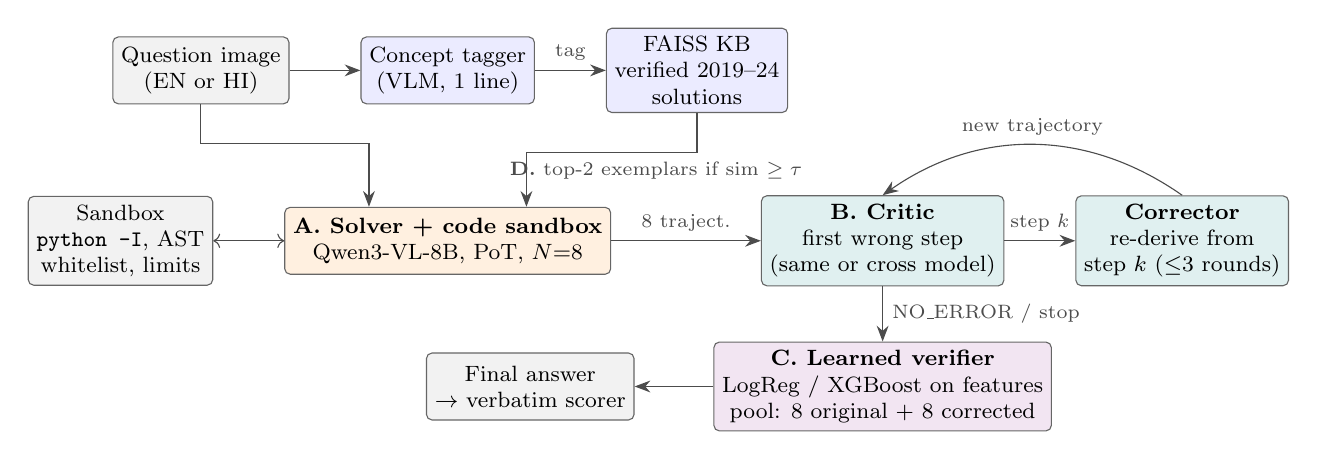
\begin{tikzpicture}[font=\footnotesize, node distance=4mm and 9mm,
  box/.style={draw=black!60, rounded corners=2pt, fill=#1, align=center, minimum height=8.5mm,
  inner sep=3pt}, box/.default=white, arr/.style={-{Stealth[length=2mm]}, black!70}]
\node[box=black!5] (img) {Question image\\(EN or HI)};
\node[box=blue!8, right=of img] (tag) {Concept tagger\\(VLM, 1 line)};
\node[box=blue!8, right=of tag] (kb) {FAISS KB\\verified 2019--24\\solutions};
\node[box=orange!12, below=13mm of tag, minimum width=34mm] (solver)
  {\textbf{A. Solver + code sandbox}\\Qwen3-VL-8B, PoT, $N{=}8$};
\node[box=black!5, left=of solver] (exec) {Sandbox\\\texttt{python -I}, AST\\whitelist, limits};
\node[box=teal!12, right=19mm of solver] (critic) {\textbf{B. Critic}\\first wrong step\\(same or cross model)};
\node[box=teal!12, right=of critic] (corr) {\textbf{Corrector}\\re-derive from\\step $k$ ($\le$3 rounds)};
\node[box=violet!10, below=7mm of critic, minimum width=40mm] (ver)
  {\textbf{C. Learned verifier}\\LogReg / XGBoost on features\\pool: 8 original + 8 corrected};
\node[box=black!5, left=10mm of ver] (out) {Final answer\\$\to$ verbatim scorer};
\draw[arr] (img) -- (tag); \draw[arr] (tag) -- node[above]{\scriptsize tag} (kb);
\draw[arr] (kb.south) -- ++(0,-5mm) -| node[pos=0.12,below]{\scriptsize \textbf{D.} top-2 exemplars if sim $\ge\tau$} ([xshift=10mm]solver.north);
\draw[arr] (img.south) -- ++(0,-5mm) -| ([xshift=-10mm]solver.north);
\draw[arr, <->] (exec) -- (solver);
\draw[arr] (solver) -- node[above]{\scriptsize 8 traject.} (critic);
\draw[arr] (critic) -- node[above]{\scriptsize step $k$} (corr);
\draw[arr] (corr.north) to[bend right=35] node[above]{\scriptsize new trajectory} (critic.north);
\draw[arr] (critic) -- node[right]{\scriptsize NO\_ERROR / stop} (ver);
\draw[arr] (ver) -- (out);
\end{tikzpicture}
\caption{Inference-time framework around a frozen VLM. Only the verifier (C) is trained, on
automatically labelled solutions of 2019--2024 questions. The KB (D) holds no 2025 question and no
near-duplicate of one.}
\label{fig:arch}
\end{figure*}

Fig.~\ref{fig:arch} shows the pipeline; prompts are listed in the appendix.

\textbf{A. Code sandbox (PoT).} The solver writes numbered ``Step $k$:'' reasoning and puts
every calculation in a \texttt{python} block. Generation stops when a block closes; the block
runs in an isolated subprocess (\texttt{python -I}, AST whitelist of math, fractions, sympy, numpy
and scipy, no file or network I/O, CPU/memory/output limits, earlier blocks replayed so variables
persist), and its output is appended as an \texttt{output} block before generation continues
(at most 3 blocks). If no \verb|\boxed{}| answer is produced, the SOP's plain-CoT fallback
answers instead.

\textbf{B. Agentic correction.} The critic receives the image, the question type and the
numbered steps, and answers \texttt{FIRST\_ERROR\_STEP:~$k$} with a reason, or
\texttt{NO\_ERROR}. A reply cut off before a verdict is completed by a short greedy continuation
after a decision cue (verdict forcing). The corrector keeps steps $1..k{-}1$, receives the
critique and re-derives from step $k$ with the sandbox. The loop stops on \texttt{NO\_ERROR}, an
answer unchanged for two rounds, or after 3 rounds. The critic is either the solver itself or
InternVL3.5-8B~\cite{internvl35}; the cross-model variant is used in the full framework.

\textbf{C. Learned verifier.} Training data: 8 PoT samples for each of the 1{,}270 training
questions (\VerN{} solutions), labelled correct/incorrect by the verbatim scorer. Features:
(i) 31 handcrafted features: length (tokens, characters, steps), code blocks run or failed,
fallback, truncation, hedging words, agreement with the sibling answers (fraction, majority,
vote rank, distinct answers), answer plausibility (numeric, integer, sign, magnitude, decimals,
valid format and letters, number of \verb|\boxed|), question type, subject, language and
diagram flag; (ii) a bge-small sentence embedding of the solution,
reduced to 32 dimensions by PCA fitted on training data. Models: logistic regression (standardised, class-balanced) and XGBoost, each on
handcrafted, embedding or all features. Model selection: GroupKFold by twin pair on 2019--2023,
dev = 2024; the primary model and selection rule (max probability or probability-weighted vote)
are chosen on dev only. At test time it selects from the 16-candidate pool (8 originals + 8
corrected); agreement features are computed within each 8-sample sub-pool to match training.

\textbf{D. Retrieval.} The VLM writes a one-line English concept tag (subject, topic, method)
for every question, so Hindi images are matched in English. The KB holds one entry per training
twin pair: VLM transcription, tag and the shortest verified-correct PoT solution (English and
code-using preferred). Tags are embedded with bge-small and searched with FAISS inside the same
subject. The top-2 entries with cosine $\ge\tau$ are added to the solver prompt as method-only
examples; $\tau$ is tuned on 2024 queries against a 2019--2023 KB.

% ----------------------------------------------------------------------------------------------
\section{Experimental setup}
\textbf{Models and decoding.} Solver, corrector and tagger: Qwen3-VL-8B-Instruct~\cite{qwen3vl}
(AWQ 4-bit); cross-model critic: InternVL3.5-8B (AWQ 4-bit). Both run with vLLM~\cite{vllm} on
one RTX 3060 (12\,GB), one model at a time. Sampling: $T{=}0.7$, top-$p$ 0.8, top-$k$ 20, at most
4{,}096 new tokens per turn, the same for every configuration. Seeds are deterministic per
question, sample and turn.

\textbf{Sample counts.} CoT: 20 samples per question (Pass@1 and SC); PoT, RAG-PoT and
corrections: 8 per question; verifier training: 8 per training question; contamination check: 1
CoT sample per question for all years.

\textbf{Engineering.} Every model call and code execution is cached in SQLite, keyed by model,
prompt, seed and settings; a crash loses at most one batch, and all evaluation runs offline from
the cache. A supervisor runs the 14 stages with retries. The full run took \TotalHours{} GPU
hours with no retry (Table~\ref{tab:compute}). The pipeline is covered by 73 automated tests,
including an end-to-end run with a mock VLM.

\textbf{Pilot and fixes.} A 40-question pilot of all modules preceded the full run and exposed
seven method-level problems (lost code state, a blocked library, critic replies without verdict,
frequent fallbacks, an under-sampled SC baseline, a weak selector, and one over-long prompt that
aborted a batch); all were fixed or, for the fallback, tested and kept (details in the Phase-2
report).

\begin{table}[t]
\centering
\footnotesize
\caption{Wall-clock time of the full run (supervisor log); no stage needed a retry.}
\label{tab:compute}
\setlength{\tabcolsep}{3.5pt}
\begin{tabular}{lr}
\toprule
Stage (one RTX 3060, 12\,GB) & Hours \\
\midrule
CoT, 20 $\times$ 190 (16 cached) & 1.5 \\
PoT, 8 $\times$ 190 & 3.3 \\
Correction, same-model critic & 5.4 \\
Correction, cross-model critic & 5.9 \\
PoT on train, 8 $\times$ 1{,}270 & 23.9 \\
RAG-PoT, 8 $\times$ 190 & 3.8 \\
Full correction (RAG-PoT) & 7.7 \\
CoT on train, 1 $\times$ 1{,}270 & 2.8 \\
\textbf{Total} & \textbf{54.4} \\
\bottomrule
\end{tabular}
\end{table}


% ----------------------------------------------------------------------------------------------
\section{Results}
\begin{table*}[t]
\centering
\footnotesize
\caption{SOP Table I: additive evaluation on the 2025 held-out set (190 questions, 95 EN + 95 HI). Pass@1 = mean over samples for single-candidate rows; the verifier rows select one answer per question. CIs: cluster bootstrap over EN/HI twins (2{,}000 resamples). Self-consistency uses the number of CoT samples whose tokens match the full framework.}
\label{tab:table1}
\setlength{\tabcolsep}{3.5pt}
\begin{tabular}{lrrcrrr}
\toprule
Configuration & Numerical & Overall & 95\% CI & $\Delta$ vs baseline [CI] & Tok/q & Calls/q \\
\midrule
Baseline CoT & 40.2 & \textbf{43.2} & [37.0, 49.6] & -- & 2.7k & 1.0 \\
Self-consistency (matched) (n=20) & 51.2 & \textbf{53.2} & [44.2, 62.6] & +10.0 [+5.3, +14.6] & 54.2k & 20.0 \\
+ Code sandbox (PoT) & 50.4 & \textbf{48.2} & [41.4, 54.9] & +5.0 [+0.4, +9.8] & 3.5k & 1.9 \\
+ Correction, same-model critic & 55.1 & \textbf{51.2} & [44.6, 58.0] & +8.1 [+3.3, +13.1] & 6.1k & 4.4 \\
+ Correction, cross-model critic & 53.0 & \textbf{51.3} & [44.5, 58.1] & +8.2 [+3.5, +13.4] & 6.4k & 4.7 \\
+ Learned verifier & 66.7 & \textbf{63.2} & [55.3, 71.6] & +20.0 [+13.4, +27.0] & 51.5k & 37.6 \\
+ RAG = Full framework & 69.0 & \textbf{65.3} & [57.4, 73.7] & +22.1 [+16.1, +28.5] & 54.1k & 39.2 \\
\bottomrule
\end{tabular}
\end{table*}


\subsection{Main result}
Table~\ref{tab:table1} and Fig.~\ref{fig:table1} give SOP Table~I. Every module adds accuracy:
the code sandbox lifts the baseline from \BaseAcc\% to \PotAcc\% (Numerical \BaseNum\%$\to$\PotNum\%),
correction adds about 3 points (\CsAcc\% same-model, \CcAcc\% cross-model), the verifier over
the 16-candidate pool reaches \VerAcc\%, and retrieval brings the full framework to
\textbf{\FullAcc\%} (Numerical \FullNum\%).

\begin{figure}[t]
\centering
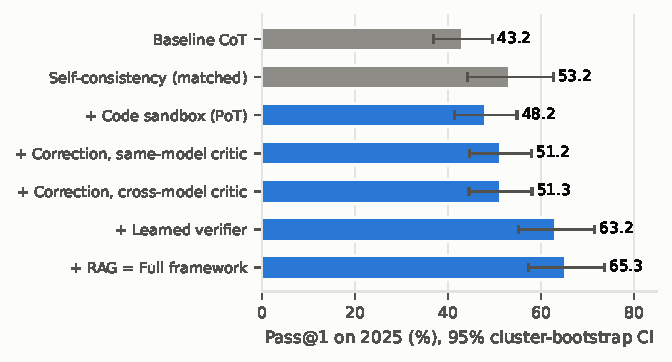
\includegraphics[width=\columnwidth]{fig_table1.pdf}
\caption{SOP Table~I on the 2025 test set with 95\% cluster-bootstrap CIs. Grey: baselines.}
\label{fig:table1}
\end{figure}

\subsection{Compute-matched comparison and significance}
The full framework generates \FullTok{} tokens per question, as much as \ScN{} CoT samples.
SC with those samples reaches \ScAcc\% (at most \ScMax\% for any $n$), so the framework is
\FullVsSc{} points better at equal compute (Fig.~\ref{fig:compute}); it answers \FullOnly{}
questions correctly that SC gets wrong, against \ScOnly{} the other way (McNemar
$p{=}$\FullVsScP). Table~\ref{tab:sig} tests each step: the sandbox, correction and the
verifier step are significant; retrieval on top of the verifier is not.

\begin{figure}[t]
\centering
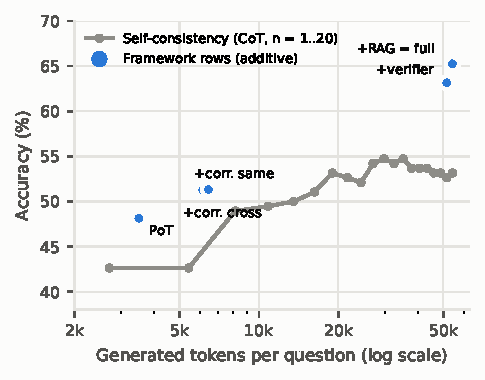
\includegraphics[width=\columnwidth]{fig_compute.pdf}
\caption{Accuracy vs.\ generated tokens per question. Grey: SC over $n$ CoT samples. Every
framework row lies above the SC curve; the full framework beats SC at equal cost.}
\label{fig:compute}
\end{figure}
\begin{table*}[t]
\centering
\footnotesize
\caption{Paired cluster-bootstrap tests of key steps; McNemar where both rows give one answer per question.}
\label{tab:sig}
\setlength{\tabcolsep}{3.5pt}
\begin{tabular}{lrrr}
\toprule
Comparison & $\Delta$ [95\% CI] & $P(\Delta\le0)$ & McNemar (a only / b only) \\
\midrule
Code sandbox (PoT) vs Baseline CoT & +5.0 [+0.4, +9.8] & 0.0120 & -- \\
Correction, cross-model critic vs Code sandbox (PoT) & +3.2 [+1.3, +5.0] & 0.0005 & -- \\
Learned verifier vs Correction, cross-model critic & +11.8 [+6.8, +16.6] & 0.0000 & -- \\
RAG = Full framework vs Learned verifier & +2.1 [-3.2, +6.8] & 0.2235 & 13 / 9, $p$=0.5235 \\
RAG = Full framework vs Self-consistency (matched) & +12.1 [+4.2, +20.0] & 0.0015 & 35 / 12, $p$=0.0011 \\
RAG = Full framework vs Baseline CoT & +22.1 [+15.9, +28.6] & 0.0000 & -- \\
\bottomrule
\end{tabular}
\end{table*}


\subsection{Where the framework helps}
\begin{table*}[t]
\centering
\footnotesize
\caption{Accuracy (\%) by question type (84 / 46 / 42 / 18 questions), language, subject and diagram dependence.}
\label{tab:breakdown}
\setlength{\tabcolsep}{3.5pt}
\begin{tabular}{lrrrrrrrrrrr}
\toprule
Configuration & Num. & MCQ-S & MCQ-M & Match. & EN & HI & Math & Chem & Phys & No diag. & Diag. \\
\midrule
Baseline CoT & 40.2 & 48.5 & 46.0 & 36.7 & 48.1 & 38.3 & 53.9 & 41.6 & 33.6 & 48.2 & 29.7 \\
Self-consistency (matched) & 51.2 & 56.5 & 54.8 & 50.0 & 57.9 & 48.4 & 70.3 & 48.4 & 40.3 & 58.7 & 38.5 \\
+ Code sandbox (PoT) & 50.4 & 51.9 & 44.9 & 35.4 & 54.7 & 41.6 & 64.6 & 42.4 & 37.1 & 54.1 & 32.5 \\
+ Correction, same-model critic & 55.1 & 52.7 & 46.4 & 41.0 & 58.0 & 44.5 & 68.8 & 44.7 & 39.9 & 58.2 & 32.9 \\
+ Correction, cross-model critic & 53.0 & 55.2 & 47.6 & 42.4 & 58.8 & 43.8 & 71.1 & 44.5 & 37.9 & 58.2 & 32.9 \\
+ Learned verifier & 66.7 & 65.2 & 54.8 & 61.1 & 72.6 & 53.7 & 76.6 & 57.8 & 54.8 & 68.8 & 48.1 \\
+ RAG = Full framework & 69.0 & 67.4 & 59.5 & 55.6 & 73.7 & 56.8 & 79.7 & 60.9 & 54.8 & 72.5 & 46.2 \\
\bottomrule
\end{tabular}
\end{table*}

\begin{figure*}[t]
\centering
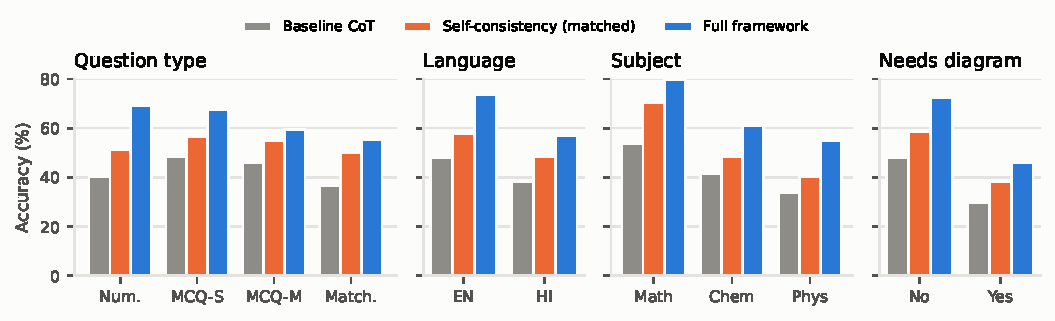
\includegraphics[width=0.95\textwidth]{fig_breakdown.pdf}
\caption{Accuracy by question type, language, subject and diagram dependence for the baseline,
compute-matched SC and the full framework.}
\label{fig:breakdown}
\end{figure*}

Gains are largest on Numerical questions (+28.8 points) and Mathematics (+25.8), where
computation dominates, and the framework beats SC on every type and subject
(Table~\ref{tab:breakdown}, Fig.~\ref{fig:breakdown}). It does not close the gaps the paper
reports: English gains more than Hindi (the gap grows from 9.8 to 16.9 points) and text-only
questions gain more than diagram questions (gap 18.5$\to$26.3). The framework improves
\emph{reasoning and computation}, not perception or Hindi reading.

\subsection{Code sandbox}
\begin{figure*}[t]
\centering
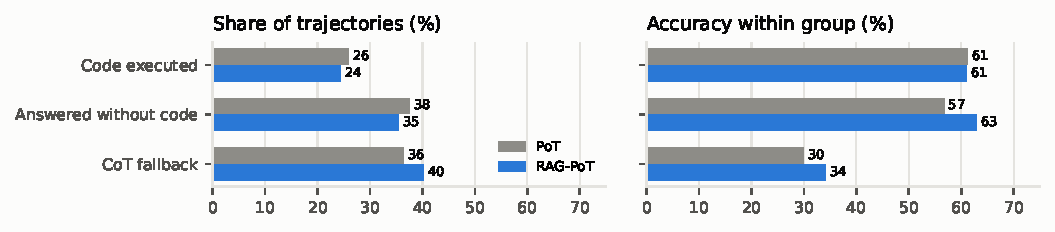
\includegraphics[width=0.92\textwidth]{fig_pot_anatomy.pdf}
\caption{PoT and RAG-PoT trajectories by outcome (share and accuracy within each group).}
\label{fig:anatomy}
\end{figure*}
Only \PotCodeRan\% of PoT trajectories execute code; another 38\% answer directly, and
\PotFallback\% run out of tokens and fall back to CoT (Fig.~\ref{fig:anatomy}). Code-executing
and direct answers are about twice as accurate as fallbacks (61\% and 57\% vs.\ 30\%). The 4{,}096-token
cap is the main remaining loss: \CotTrunc\% of CoT samples and \PotTrunc\% of PoT trajectories
hit it, mostly in loops of re-checking (Fig.~\ref{fig:tokens}).

\begin{figure*}[t]
\centering
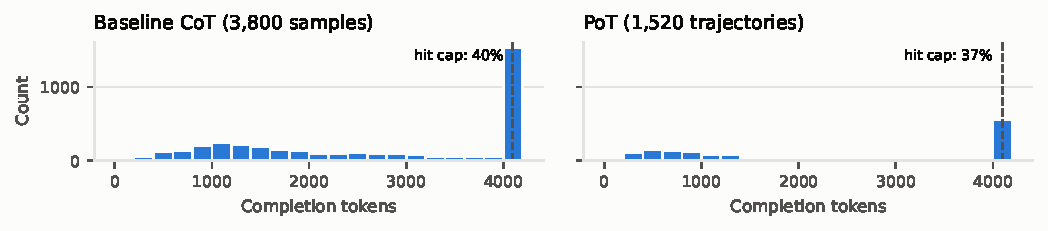
\includegraphics[width=0.92\textwidth]{fig_tokens.pdf}
\caption{Completion lengths; the dashed line is the 4{,}096-token cap.}
\label{fig:tokens}
\end{figure*}

\subsection{Agentic correction}
\begin{table*}[t]
\centering
\footnotesize
\caption{Agentic correction. Detect = critic flags an originally wrong solution; False al. = flags a correct one; Fix$|$det. = detected wrong solutions that end correct.}
\label{tab:correction}
\setlength{\tabcolsep}{3.5pt}
\begin{tabular}{lrrrrrrr}
\toprule
Run (1{,}520 chains) & Acc. before $\to$ after & Detect & False al. & Fix$|$det. & W$\to$R / R$\to$W & Rounds & Stop: ok / unch. / max \\
\midrule
Same-model critic, PoT source & 48.2 $\to$ 51.2 & 57.9 & 19.3 & 14.3 & 65 / 18 & 1.47 & 1151 / 308 / 61 \\
Cross-model critic, PoT source & 48.2 $\to$ 51.3 & 59.3 & 25.7 & 18.6 & 87 / 39 & 1.53 & 1137 / 328 / 55 \\
Cross-model critic, RAG-PoT source & 50.9 $\to$ 54.7 & 60.7 & 28.6 & 19.2 & 87 / 29 & 1.53 & 1124 / 345 / 51 \\
Base paper (single pass, EP$\to$EC) &  &  &  & 1.1--5.2 &  & 1 &  \\
\bottomrule
\end{tabular}
\end{table*}

\begin{figure*}[t]
\centering
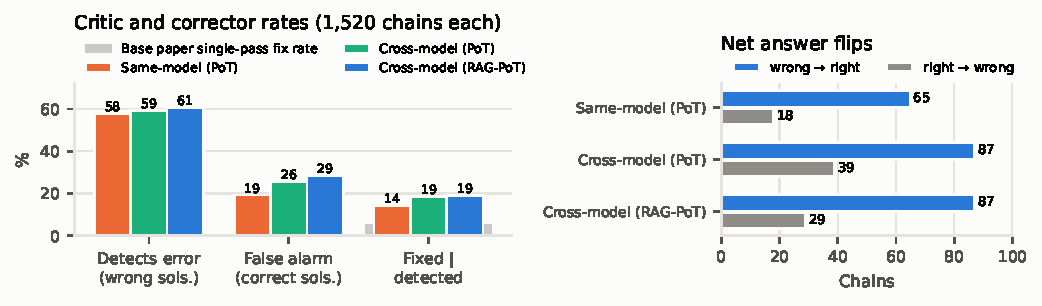
\includegraphics[width=0.95\textwidth]{fig_correction.pdf}
\caption{Correction loop on 1{,}520 chains per run. Left: detection, false alarms and fixes of
detected errors (grey band: the paper's single-pass 1.1--5.2\%). Right: answer flips.}
\label{fig:correction}
\end{figure*}

Critics flag about 60\% of wrong solutions; step-localised, multi-round correction then fixes
\FixSame--\FixFull\% of them, 3--17$\times$ the paper's single-pass rate
(Table~\ref{tab:correction}, Fig.~\ref{fig:correction}). The cross-model critic fixes more
(87 vs.\ 65 wrong$\to$right) but raises more false alarms and breaks more correct answers
(39 vs.\ 18), so both critics give the same net gain of about 3 points. Most chains stop after
one or two rounds because the critic accepts the solution. Detection is no longer the bottleneck;
turning a detected error into a correct answer is.

\subsection{Learned verifier}
\begin{table*}[t]
\centering
\footnotesize
\caption{Learned verifier trained on 10,160 auto-labelled solutions of 1,270 training questions (45.5\% correct). CV: GroupKFold by twin pair on 2019--2023; dev: 2024; test: the 2025 full pool (16 candidates per question). Sel.\ = accuracy of the max-probability candidate. $^\star$ = primary model, chosen on dev only.}
\label{tab:verifier}
\setlength{\tabcolsep}{3.5pt}
\begin{tabular}{lrrrrrrrr}
\toprule
Model / features & CV AUC & CV F1 & Dev AUC & Dev F1 & Dev sel. & Test AUC & Test F1 & Test sel. \\
\midrule
LR / handcrafted & 0.893 & 0.796 & 0.916 & 0.844 & 60.3 & 0.838 & 0.776 & 64.2 \\
LR / embedding & 0.672 & 0.641 & 0.706 & 0.698 & 50.0 & 0.652 & 0.688 & 59.5 \\
LR / all $^\star$ & 0.891 & 0.794 & 0.915 & 0.847 & 61.8 & 0.836 & 0.774 & 65.3 \\
XGB / handcrafted & 0.901 & 0.801 & 0.913 & 0.831 & 59.3 & 0.889 & 0.802 & 67.4 \\
XGB / embedding & 0.677 & 0.646 & 0.689 & 0.687 & 51.5 & 0.640 & 0.694 & 52.1 \\
XGB / all & 0.902 & 0.804 & 0.911 & 0.819 & 59.8 & 0.882 & 0.815 & 67.9 \\
\midrule
Majority vote &  &  &  &  & 59.3 &  &  & 65.8 \\
Oracle (any correct) &  &  &  &  & 77.0 &  &  & 85.3 \\
\bottomrule
\end{tabular}
\end{table*}

\begin{figure}[t]
\centering
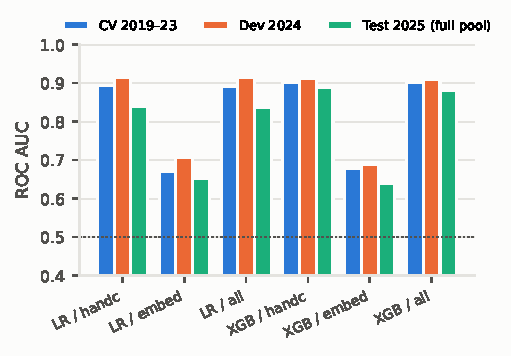
\includegraphics[width=\columnwidth]{fig_verifier_auc.pdf}
\caption{Verifier ROC AUC: cross-validation, dev year and the 2025 full pool.}
\label{fig:verauc}
\end{figure}
\begin{figure*}[t]
\centering
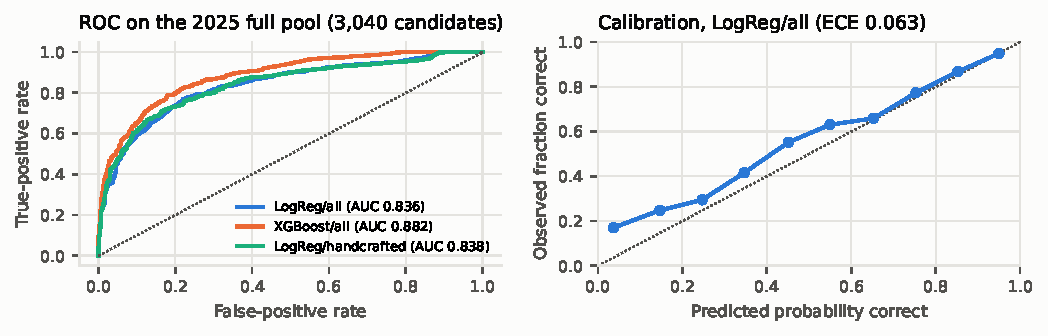
\includegraphics[width=0.92\textwidth]{fig_verifier_roc.pdf}
\caption{Verifier on the 2025 full pool. Left: ROC curves. Right: reliability of the primary
model's probabilities (10 bins).}
\label{fig:verroc}
\end{figure*}

\textbf{As a classifier} the verifier works (Table~\ref{tab:verifier}, Figs.~\ref{fig:verauc},
\ref{fig:verroc}): AUC \VerDevAuc{} on the dev year and \VerTestAuc{} on 2025 for the primary
model (\XgbTestAuc{} for XGBoost), with reasonable calibration (ECE \Ece). Handcrafted features
carry the signal; the embedding alone reaches only 0.64--0.71. The most important features
(Fig.~\ref{fig:coef}) are agreement with sibling answers, a valid answer format and length;
truncation and the CoT fallback lower the predicted probability. Length features are correlated
(\texttt{log\_tokens} vs.\ \texttt{log\_chars}), so their signs should not be read in isolation.

\begin{figure}[t]
\centering
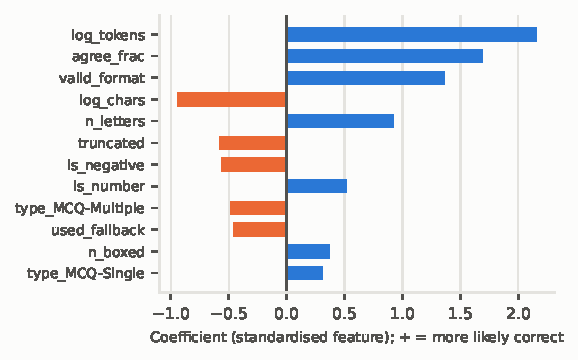
\includegraphics[width=\columnwidth]{fig_verifier_coef.pdf}
\caption{Largest coefficients of the logistic-regression verifier on standardised handcrafted
features.}
\label{fig:coef}
\end{figure}

\begin{table*}[t]
\centering
\footnotesize
\caption{Answer selection on the 2025 pools (accuracy \%). $^\star$ = primary verifier chosen on 2024. Reported only; no choice was made on 2025.}
\label{tab:selection}
\setlength{\tabcolsep}{3.5pt}
\begin{tabular}{lrrrrrr}
\toprule
2025 candidate pool & Majority & LR max-p.$^\star$ & LR w.-vote & XGB max-p. & Oracle & LR AUC \\
\midrule
8 PoT samples & 60.5 & 61.6 & 61.6 & 65.3 & 78.9 & 0.834 \\
8 PoT + 8 corrected (cross) & 61.6 & 63.2 & 63.2 & 66.8 & 82.6 & 0.828 \\
8 RAG-PoT + 8 corrected (full) & 65.8 & 65.3 & 66.8 & 67.9 & 85.3 & 0.836 \\
\bottomrule
\end{tabular}
\end{table*}

\begin{figure}[t]
\centering
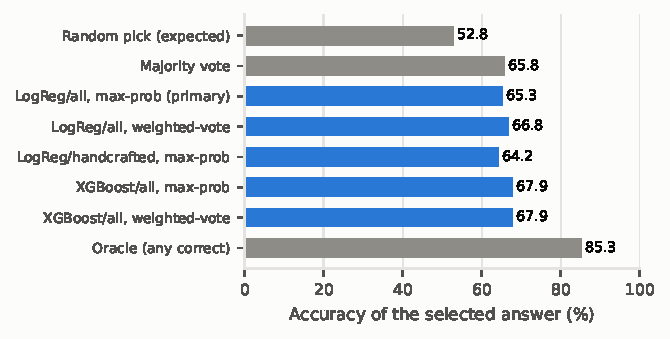
\includegraphics[width=\columnwidth]{fig_selection.pdf}
\caption{Accuracy of the selected answer on the 2025 full pool for different selectors.}
\label{fig:selection}
\end{figure}

\textbf{As a selector} it is honest to separate two effects (Table~\ref{tab:selection},
Fig.~\ref{fig:selection}). Pooling 16 diverse candidates already raises majority-vote accuracy
to \SelMaj\% on the full pool (from 53.2\% for 20 CoT votes), so most of the jump in
Table~\ref{tab:table1} comes from the \emph{candidate pool}, not from the classifier. The primary
verifier, chosen on 2024 where it beat majority voting (61.8\% vs.\ 59.3\%), selects
\SelPrim\% on 2025, the same as majority voting within noise. XGBoost would have reached
\SelXgb\%, but it was not the dev choice, and we do not select on test data. The oracle
(\SelOracle\%) shows that a better selector could still add up to 20 points.

\subsection{Retrieval}
\begin{table}[t]
\centering
\footnotesize
\caption{RAG knowledge base and the effect of retrieval on PoT accuracy.}
\label{tab:rag}
\setlength{\tabcolsep}{3.5pt}
\begin{tabular}{lr}
\toprule
Retrieval (full run) & Value \\
\midrule
Training twin pairs (2019--2024) & 635 \\
No verified-correct solution & 180 \\
Near-duplicate of a 2025 question & 1 \\
KB entries & 454 \\
Threshold $\tau$ (tuned on 2024) & 0.885 \\
Dev proxy precision (base rate) & 70.6\% (31.4\%) \\
2025 questions with exemplars & 30 / 190 \\
PoT $\to$ RAG-PoT, with exemplars & 30.0 $\to$ 37.9 \\
PoT $\to$ RAG-PoT, without exemplars & 51.6 $\to$ 53.4 \\
\bottomrule
\end{tabular}
\end{table}

\begin{figure}[t]
\centering
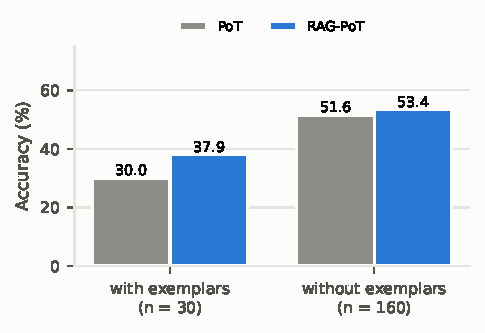
\includegraphics[width=\columnwidth]{fig_rag.pdf}
\caption{PoT vs.\ RAG-PoT accuracy for test questions that did and did not receive exemplars.
Without exemplars the prompt is unchanged, so that difference is sampling noise.}
\label{fig:rag}
\end{figure}
The KB holds \KbEntries{} verified solutions. The tuned threshold favours precision, so only
\RagN{} of 190 test questions receive exemplars (Table~\ref{tab:rag}). On those, which are
harder than average, RAG-PoT improves from \RagWithPot\% to \RagWithRag\%; on the others the
prompt is unchanged and the change (\RagWoPot\%$\to$\RagWoRag\%) is sampling noise
(Fig.~\ref{fig:rag}). Overall RAG-PoT reaches \RagMean\% vs.\ \PotAcc\% for PoT, and +2.1
points in the full framework, which is not significant (Table~\ref{tab:sig}). Retrieval helps
when a close match exists, but its coverage limits the effect.

\subsection{Contamination check}
\begin{figure}[t]
\centering
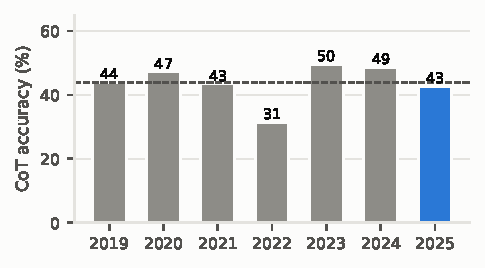
\includegraphics[width=\columnwidth]{fig_contamination.pdf}
\caption{Baseline CoT accuracy (1 sample per question) per exam year; dashed: 2019--2024 mean.}
\label{fig:contam}
\end{figure}
Qwen3-VL was released after the 2025 exam. Following the paper's check, one CoT sample per
question scores \ConTrain\% on 2019--2024 and \ConTest\% on 2025 (\ConDelta{} points;
Fig.~\ref{fig:contam}). Older, more likely memorised years are not easier, so there is no sign
of memorisation; exposure to 2025 itself cannot be ruled out completely.

\subsection{Reproduction of the base paper}
With the paper's prompts and scorer, Qwen2.5-VL-7B scores \ReproAcc\,$\pm$\,\ReproStd\% over 10
runs vs.\ 12.4\,$\pm$\,1.9\% in the paper, so the harness matches the original protocol and the
much higher Qwen3-VL-8B baseline is a model effect, not an evaluation artefact.

% ----------------------------------------------------------------------------------------------
\section{Discussion}
\textbf{What worked.} Moving computation into code and sampling several code-based candidates,
then correcting them and choosing among them, gives a large and significant gain over voting on
plain CoT at the same cost. Step-localised, multi-round correction turns detections into fixes
far more often than the paper's single pass.

\textbf{What did not work as hoped.} (i) The learned verifier is a good classifier but, on 2025,
not a better selector than majority voting over the same pool; with a stronger dev signal (or a
selector trained directly for ranking) the oracle gap of about 20 points is the largest
opportunity. (ii) Retrieval is limited by coverage: only 16\% of test questions found a close
match. (iii) A cross-model critic finds more errors but also breaks more correct answers, so it
did not beat self-critique in net accuracy.

\textbf{Remaining failure modes.} 37--40\% of trajectories hit the token cap, and accuracy on
diagram questions and Hindi questions improves less than on text and English questions. These
are perception and reading problems that inference-time reasoning does not solve.

\section{Limitations and threats to validity}
One substrate model and one test year (190 questions; CIs about $\pm$8 points). 4-bit weights and
a fixed 4{,}096-token budget. Compute matching counts generated tokens, not prompt tokens or the
cost of code execution. The unchanged scorer gives no partial credit and reads only the first
\verb|\boxed{}|. Exposure of Qwen3-VL to the 2025 exam cannot be excluded completely.

\section{Conclusion}
A frozen 8B VLM with a code sandbox, step-localised correction, a light learned verifier and
retrieval improves mmJEE-Eval 2025 accuracy from \BaseAcc\% to \FullAcc\% and beats
compute-matched self-consistency by \FullVsSc{} points, without any fine-tuning. The analysis
points to two next steps: a selector that closes the gap to the oracle, and fixing truncation and
perception, which no amount of reasoning-time compute addresses.

\clearpage
\appendices
\section{Prompts}
The prompts below are generated from the code (\texttt{prompts/templates.py}); the baseline
prompt is the paper's (Appendix C), and the Hindi variant is analogous.
{\footnotesize \paragraph{Baseline (base paper, English)}
\begin{small}\begin{verbatim}
Please analyze the image carefully, reason
step-by-step and provide your answer at the
end.

For this question:
- Provide a numerical value
- Round to appropriate decimal places if
needed
- Format your answer in \boxed{} (e.g.,
\boxed{2.5} or \boxed{42})
\end{verbatim}\end{small}

\paragraph{PoT solver instructions}
\begin{small}\begin{verbatim}
How to solve:
- Write the solution as numbered steps, each
starting on a new line with "Step 1:", "Step
2:", and so on.
- Explain the physics/chemistry/mathematics of
each step in words.
- Do NOT do calculations in your head.
Whenever a step needs a calculation
(arithmetic, algebra, solving equations,
derivatives, integrals, limits, unit
conversions, or checking each option), write a
short Python program in a ```python code block
that prints the result. You may use math,
fractions, sympy and numpy.
- End the code block with ```. The code will
be run and its printed output will be given
back to you in an ```output block. Then
continue the solution using that output. Never
invent the output yourself.
- Use at most 3 code blocks.
- Be concise: do not re-check the same step
again and again.
- Finish with exactly one final answer in
\boxed{}. Do not use \boxed anywhere else. For
a numerical answer write a plain decimal
number inside the box (no units, no fractions,
no LaTeX), rounded to two decimal places if it
is not an integer.

Required format (example):
Step 1: <which law / concept applies and the
equation to use>
```python
import sympy as sp
x = sp.symbols('x')
print(sp.solve(2*x - 6, x))
```
```output
[3]
```
Step 2: <interpret the printed result, check
the options>
\boxed{<answer>}
\end{verbatim}\end{small}

\paragraph{Critic}
\begin{small}\begin{verbatim}
You are a strict examiner checking a student's
solution to a JEE Advanced question. The
question is in the attached image{lang_note}.

Instructions the student was given:
{type_instruction}

Student's solution (steps are numbered):
<solution>
{solution}
</solution>

Check the steps in order: reading of the
question and figure, chosen concept and
equations, algebra and arithmetic (the
```output blocks are real program outputs),
and the final option or number. Find the FIRST
step that contains an error. Do not solve the
whole problem again. Keep your check short (at
most about 250 words), then end your reply
with exactly these three lines:
VERDICT: CORRECT or ERROR
FIRST_ERROR_STEP: <step number, or NONE>
EXPLANATION: <one or two sentences: what is
wrong and how to fix it>
\end{verbatim}\end{small}

\paragraph{Corrector feedback}
\begin{small}\begin{verbatim}
A reviewer checked an earlier attempt at this
question. The steps before Step {k} were
accepted and are already written at the start
of your answer. The reviewer found an error in
Step {k}:
"{explanation}"
Continue the solution from Step {k}: re-derive
that step correctly (do not repeat the error)
and complete the solution, following the same
rules (Python code for every calculation, one
final \boxed{{}} answer).
\end{verbatim}\end{small}

\paragraph{Concept tagger}
\begin{small}\begin{verbatim}
Look at this JEE Advanced exam question (it
may be written in English or Hindi). Do not
solve it. In English, describe what is needed
to solve it, using exactly this format on one
line:
SUBJECT: <Physics/Chemistry/Mathematics> |
TOPIC: <specific topic, 2-6 words> | METHOD:
<key concept or solution technique, at most 15
words>
\end{verbatim}\end{small}

\paragraph{Transcriber}
\begin{small}\begin{verbatim}
Transcribe this exam question exactly as plain
text in its original language. Write
mathematical expressions in LaTeX. Include all
answer options. If there is a figure, add one
line "[Figure: <short description>]". Output
only the transcription.
\end{verbatim}\end{small}

\paragraph{Exemplar header}
\begin{small}\begin{verbatim}
Below are worked solutions of earlier JEE
Advanced problems that use a similar method.
Use them only as guidance on the method. They
are DIFFERENT problems: do not copy their
numbers or answers.
\end{verbatim}\end{small}
}

\section{Reproducibility}
All code, configuration and tests are in \texttt{mmjee-reasoner/}. \texttt{scripts/lab/launch.sh}
runs the full pipeline under the supervisor; \texttt{mmjee evaluate} and \texttt{mmjee report}
recompute every table from the cache; \texttt{scripts/final\_report.py} produces the figures and
tables of this report. Seeds are fixed per question, sample and turn, so re-runs hit the cache
and give identical results.

\begin{thebibliography}{99}\footnotesize
\bibitem{mmjee} A.~Mukherjee and S.~Ghosh, ``mmJEE-Eval: A bilingual multimodal benchmark for
evaluating scientific reasoning in vision-language models,'' in \emph{Proc.\ IJCNLP-AACL}, 2025.
\bibitem{selfconsistency} X.~Wang \emph{et al.}, ``Self-consistency improves chain of thought
reasoning in language models,'' in \emph{Proc.\ ICLR}, 2023.
\bibitem{pot} W.~Chen \emph{et al.}, ``Program of thoughts prompting: Disentangling computation
from reasoning for numerical reasoning tasks,'' \emph{TMLR}, 2023.
\bibitem{pal} L.~Gao \emph{et al.}, ``PAL: Program-aided language models,'' in \emph{Proc.\
ICML}, 2023.
\bibitem{selfrefine} A.~Madaan \emph{et al.}, ``Self-Refine: Iterative refinement with
self-feedback,'' in \emph{Proc.\ NeurIPS}, 2023.
\bibitem{critic} Z.~Gou \emph{et al.}, ``CRITIC: Large language models can self-correct with
tool-interactive critiquing,'' in \emph{Proc.\ ICLR}, 2024.
\bibitem{cannotselfcorrect} J.~Huang \emph{et al.}, ``Large language models cannot self-correct
reasoning yet,'' in \emph{Proc.\ ICLR}, 2024.
\bibitem{cobbe} K.~Cobbe \emph{et al.}, ``Training verifiers to solve math word problems,''
arXiv:2110.14168, 2021.
\bibitem{lightman} H.~Lightman \emph{et al.}, ``Let's verify step by step,'' in \emph{Proc.\
ICLR}, 2024.
\bibitem{rag} P.~Lewis \emph{et al.}, ``Retrieval-augmented generation for knowledge-intensive
NLP tasks,'' in \emph{Proc.\ NeurIPS}, 2020.
\bibitem{faiss} J.~Johnson, M.~Douze and H.~J\'egou, ``Billion-scale similarity search with
GPUs,'' \emph{IEEE Trans.\ Big Data}, 2019.
\bibitem{bge} S.~Xiao \emph{et al.}, ``C-Pack: Packed resources for general Chinese
embeddings,'' in \emph{Proc.\ SIGIR}, 2024.
\bibitem{vllm} W.~Kwon \emph{et al.}, ``Efficient memory management for large language model
serving with PagedAttention,'' in \emph{Proc.\ SOSP}, 2023.
\bibitem{qwen3vl} Qwen Team, ``Qwen3-VL,'' model release and technical report, 2025.
\bibitem{internvl35} OpenGVLab, ``InternVL3.5,'' model release and technical report, 2025.
\end{thebibliography}
\end{document}
